
Consider the function $$f(x_1,x_2)=\frac{1}{2}x_1^2+x_1 \cos x_2$$ illustrated in the figures below.

\begin{center}
  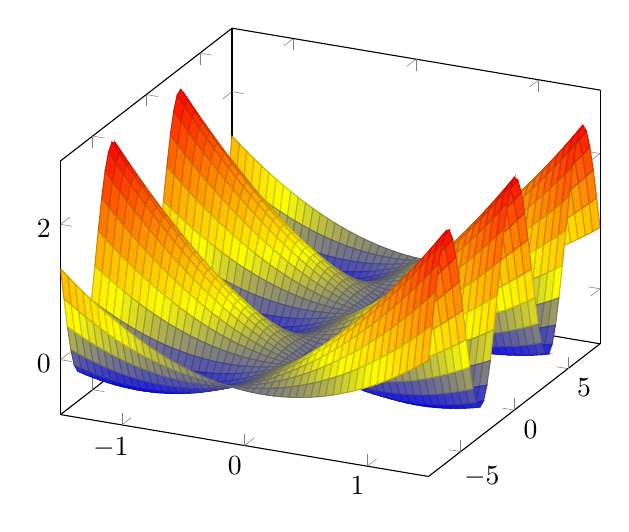
\begin{tikzpicture}
      \begin{axis}[domain=-1.5:1.5, domain y=-8:8]
     \addplot3[surf,samples=51]
      {0.5*x^2+x*cos(deg(y))};
      \end{axis}
   \end{tikzpicture}
\end{center}

\begin{center}
  \begin{tikzpicture}
      \begin{axis}[view={0}{90},domain=-1.5:1.5, domain y=-8:8]
     \addplot3[contour gnuplot={labels=false,number=40,handler/.style=smooth},samples=51]
      {0.5*x^2+x*cos(deg(y))};
      \end{axis}
   \end{tikzpicture}
\end{center}



Use the optimality conditions to identify the minima of this function.


